\documentclass[leqno]{article}
\usepackage[utf8]{inputenc}
\usepackage{enumitem}
\usepackage{tikz}
\usepackage[parfill]{parskip} % Don't start new paragraph with tab.
\usepackage{amsmath} % For \tag and \eqref

\title{Computationele logica}
\author{
    Kamans, Jim\\
    \texttt{10302905}
    \and
    Roosingh, Sander\\
    \texttt{11983957}
    \and
    Schenk, Stefan\\
    \texttt{11881798}
}
\date{November 2017}

\begin{document}

\maketitle


%%%%%%%%%%%%%%%%
%% Exercise 1 %%
%%%%%%%%%%%%%%%%
\section*{Exercise 1}

\begin{enumerate}

    \item The sentence $\theta$ encoding all information: \\

    The Queen knows the following: \\
    Alice knows Bob has a red hat. Alice knows Bob doesn't know it, and she
    knows the Queen knows this. Alice doesn't know her own hat. \\
    Bob knows Alice has a red hat. Bob knows Alice doesn't know it, and he
    knows the Queen knows this. Bob doesn't know his own hat. \\

    $\theta$ =
        $K_q (
        K_a (
            r_b \wedge
            \neg K_b (r_b \vee w_b) \wedge
            K_q ((r_a \vee r_w) \wedge (r_b \vee r_w))
        )
        \wedge \neg K_a (r_a \vee w_a)
        \wedge
        K_b (
            r_a \wedge
            \neg K_a (r_a \vee w_a) \wedge
            K_q ((r_a \vee r_w) \wedge (r_b \vee r_w))
        )
        \wedge \neg K_b (r_b \vee w_b)
        )$

    \item A representation of the situation model \textbf{M}: \\

    $\mathcal{A}$ = \{a, b, q\} the agents Alice, Bob, and the Queen \\
    $\Phi$ = $\{r_a, w_a, r_b, w_b\}$ written as WR for:
    a is white and b is red \\

    \begin{center}
    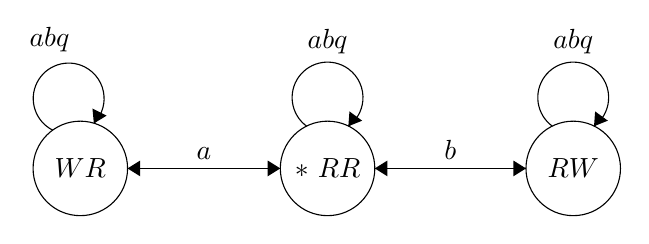
\begin{tikzpicture}[scale=0.2]
    \tikzstyle{every node}+=[inner sep=0pt]
    \draw [black] (38.4,-13.7) circle (3);
    \draw (38.4,-13.7) node {$*\mbox{ }RR$};
    \draw [black] (54,-13.7) circle (3);
    \draw (54,-13.7) node {$RW$};
    \draw [black] (22.7,-13.7) circle (3);
    \draw (22.7,-13.7) node {$WR$};
    \draw [black] (41.4,-13.7) -- (51,-13.7);
    \fill [black] (51,-13.7) -- (50.2,-13.2) -- (50.2,-14.2);
    \draw (46.2,-13.2) node [above] {$b$};
    \draw [black] (51,-13.7) -- (41.4,-13.7);
    \fill [black] (41.4,-13.7) -- (42.2,-14.2) -- (42.2,-13.2);
    \draw [black] (35.4,-13.7) -- (25.7,-13.7);
    \fill [black] (25.7,-13.7) -- (26.5,-14.2) -- (26.5,-13.2);
    \draw (30.55,-13.2) node [above] {$a$};
    \draw [black] (25.7,-13.7) -- (35.4,-13.7);
    \fill [black] (35.4,-13.7) -- (34.6,-13.2) -- (34.6,-14.2);
    \draw [black] (37.077,-11.02) arc (234:-54:2.25);
    \draw (38.4,-6.45) node [above] {$abq$};
    \fill [black] (39.72,-11.02) -- (40.6,-10.67) -- (39.79,-10.08);
    \draw [black] (52.677,-11.02) arc (234:-54:2.25);
    \draw (54,-6.45) node [above] {$abq$};
    \fill [black] (55.32,-11.02) -- (56.2,-10.67) -- (55.39,-10.08);
    \draw [black] (20.955,-11.274) arc (243.46232:-44.53768:2.25);
    \draw (20.74,-6.36) node [above] {$abq$};
    \fill [black] (23.56,-10.84) -- (24.37,-10.35) -- (23.47,-9.9);
    \end{tikzpicture}
    \end{center}

    This is an epistemic model: YES \\

    \pagebreak

    \item Seperately a and b look in their mirrors and see their red hats, the
    queen sees everything, represented in the event model $\Sigma$ with four
    actions: \\

    \begin{center}
    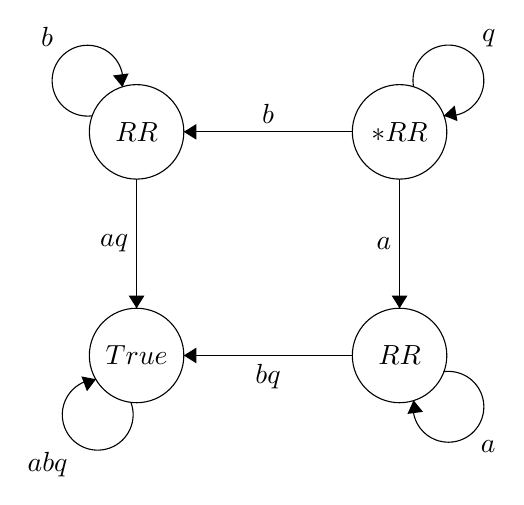
\begin{tikzpicture}[scale=0.2]
    \tikzstyle{every node}+=[inner sep=0pt]
    \draw [black] (54,-42.2) circle (3);
    \draw (54,-42.2) node {$RR$};
    \draw [black] (37.3,-28) circle (3);
    \draw (37.3,-28) node {$RR$};
    \draw [black] (37.3,-42.2) circle (3);
    \draw (37.3,-42.2) node {$True$};
    \draw [black] (54,-28) circle (3);
    \draw (54,-28) node {$*RR$};
    \draw [black] (56.805,-43.229) arc (97.58097:-190.41903:2.25);
    \draw (59.62,-47.57) node [below] {$a$};
    \fill [black] (54.89,-45.05) -- (54.5,-45.91) -- (55.49,-45.78);
    \draw [black] (34.491,-26.979) arc (277.76012:-10.23988:2.25);
    \draw (31.61,-22.64) node [above] {$b$};
    \fill [black] (36.4,-25.15) -- (36.79,-24.29) -- (35.8,-24.42);
    \draw [black] (51,-42.2) -- (40.3,-42.2);
    \fill [black] (40.3,-42.2) -- (41.1,-42.7) -- (41.1,-41.7);
    \draw (45.65,-42.7) node [below] {$bq$};
    \draw [black] (37.3,-31) -- (37.3,-39.2);
    \fill [black] (37.3,-39.2) -- (37.8,-38.4) -- (36.8,-38.4);
    \draw (36.8,-35.1) node [left] {$aq$};
    \draw [black] (51,-28) -- (40.3,-28);
    \fill [black] (40.3,-28) -- (41.1,-28.5) -- (41.1,-27.5);
    \draw (45.65,-27.5) node [above] {$b$};
    \draw [black] (54,-31) -- (54,-39.2);
    \fill [black] (54,-39.2) -- (54.5,-38.4) -- (53.5,-38.4);
    \draw (53.5,-35.1) node [left] {$a$};
    \draw [black] (54.889,-25.147) arc (190.43418:-97.56582:2.25);
    \draw (59.67,-22.63) node [above] {$q$};
    \fill [black] (56.81,-26.97) -- (57.68,-27.32) -- (57.5,-26.33);
    \draw [black] (36.935,-45.166) arc (20.7166:-267.2834:2.25);
    \draw (31.65,-48.34) node [below] {$abq$};
    \fill [black] (34.72,-43.71) -- (33.8,-43.53) -- (34.15,-44.47);
    \end{tikzpicture}
    \end{center}

    This is an epistemic model: NO \\
    This is a doxasic model: YES \\

    \item The update product of the two models \textbf{M}
    $\bigotimes$ $\Sigma$ : \\

    \begin{center}
    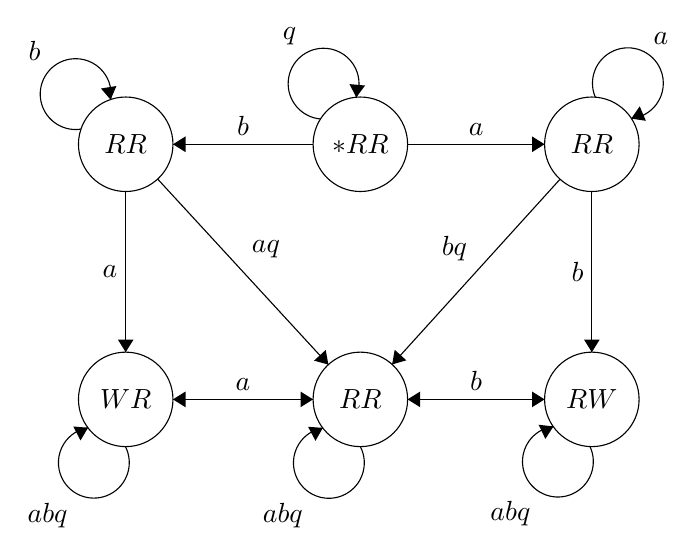
\begin{tikzpicture}[scale=0.2]
    \tikzstyle{every node}+=[inner sep=0pt]
    \draw [black] (8.5,-48.9) circle (3);
    \draw (8.5,-48.9) node {$WR$};
    \draw [black] (23.4,-48.9) circle (3);
    \draw (23.4,-48.9) node {$RR$};
    \draw [black] (38.1,-48.9) circle (3);
    \draw (38.1,-48.9) node {$RW$};
    \draw [black] (8.5,-32.7) circle (3);
    \draw (8.5,-32.7) node {$RR$};
    \draw [black] (23.4,-32.7) circle (3);
    \draw (23.4,-32.7) node {$*RR$};
    \draw [black] (38.1,-32.7) circle (3);
    \draw (38.1,-32.7) node {$RR$};
    \draw [black] (8.476,-51.888) arc (27.27123:-260.72877:2.25);
    \draw (3.54,-55.44) node [below] {$abq$};
    \fill [black] (6.11,-50.7) -- (5.17,-50.62) -- (5.63,-51.51);
    \draw [black] (23.394,-51.888) arc (27.62144:-260.37856:2.25);
    \draw (18.48,-55.46) node [below] {$abq$};
    \fill [black] (21.02,-50.71) -- (20.08,-50.64) -- (20.55,-51.53);
    \draw [black] (37.977,-51.886) arc (25.36938:-262.63062:2.25);
    \draw (32.93,-55.33) node [below] {$abq$};
    \fill [black] (35.66,-50.62) -- (34.72,-50.51) -- (35.15,-51.41);
    \draw [black] (26.4,-48.9) -- (35.1,-48.9);
    \fill [black] (35.1,-48.9) -- (34.3,-48.4) -- (34.3,-49.4);
    \draw (30.75,-48.4) node [above] {$b$};
    \draw [black] (20.4,-48.9) -- (11.5,-48.9);
    \fill [black] (11.5,-48.9) -- (12.3,-49.4) -- (12.3,-48.4);
    \draw (15.95,-48.4) node [above] {$a$};
    \draw [black] (11.5,-48.9) -- (20.4,-48.9);
    \fill [black] (20.4,-48.9) -- (19.6,-48.4) -- (19.6,-49.4);
    \draw [black] (35.1,-48.9) -- (26.4,-48.9);
    \fill [black] (26.4,-48.9) -- (27.2,-49.4) -- (27.2,-48.4);
    \draw [black] (8.5,-35.7) -- (8.5,-45.9);
    \fill [black] (8.5,-45.9) -- (9,-45.1) -- (8,-45.1);
    \draw (8,-40.8) node [left] {$a$};
    \draw [black] (5.671,-31.737) arc (278.9367:-9.0633:2.25);
    \draw (2.71,-27.44) node [above] {$b$};
    \fill [black] (7.54,-29.87) -- (7.91,-29) -- (6.93,-29.16);
    \draw [black] (20.4,-32.7) -- (11.5,-32.7);
    \fill [black] (11.5,-32.7) -- (12.3,-33.2) -- (12.3,-32.2);
    \draw (15.95,-32.2) node [above] {$b$};
    \draw [black] (20.879,-31.095) arc (265.25323:-22.74677:2.25);
    \draw (18.9,-26.43) node [above] {$q$};
    \fill [black] (23.14,-29.72) -- (23.7,-28.97) -- (22.71,-28.88);
    \draw [black] (26.4,-32.7) -- (35.1,-32.7);
    \fill [black] (35.1,-32.7) -- (34.3,-32.2) -- (34.3,-33.2);
    \draw (30.75,-32.2) node [above] {$a$};
    \draw [black] (38.325,-29.72) arc (203.42077:-84.57923:2.25);
    \draw (42.48,-26.39) node [above] {$a$};
    \fill [black] (40.6,-31.07) -- (41.53,-31.21) -- (41.14,-30.29);
    \draw [black] (38.1,-35.7) -- (38.1,-45.9);
    \fill [black] (38.1,-45.9) -- (38.6,-45.1) -- (37.6,-45.1);
    \draw (37.6,-40.8) node [left] {$b$};
    \draw [black] (10.53,-34.91) -- (21.37,-46.69);
    \fill [black] (21.37,-46.69) -- (21.2,-45.76) -- (20.46,-46.44);
    \draw (16.48,-39.34) node [right] {$aq$};
    \draw [black] (36.08,-34.92) -- (25.42,-46.68);
    \fill [black] (25.42,-46.68) -- (26.32,-46.42) -- (25.58,-45.75);
    \draw (30.21,-39.34) node [left] {$bq$};
    \end{tikzpicture}
    \end{center}

    This is an epistemic model: NO \\
    This is a doxasic model: YES \\

\end{enumerate}


%%%%%%%%%%%%%%%%
%% Exercise 2 %%
%%%%%%%%%%%%%%%%
\section*{Exercise 2}
We mark real worlds/events with an $*$.
\begin{enumerate}

    \item Representation of the bits world as an epistemic model \textbf{M}:

	\begin{center}
	\begin{tikzpicture}[scale=0.2]
		\tikzstyle{every node}+=[inner sep=0pt]
		\draw [black] (33.9,-28.5) circle (3);
		\draw (33.9,-28.5) node {$1,0,1$};
		\draw (30.4,-28.5) node {$*$};
		\draw [black] (33.9,-9.8) circle (3);
		\draw (33.9,-9.8) node {$0,0,0$};
		\draw [black] (52.4,-39.5) circle (3);
		\draw (52.4,-39.5) node {$1,1,0$};
		\draw [black] (14.1,-39.5) circle (3);
		\draw (14.1,-39.5) node {$0,1,1$};
		\draw [black] (36.045,-30.58) arc (73.6189:-214.3811:2.25);
		\draw (38.36,-35.43) node [below] {$a,b,c$};
		\fill [black] (33.55,-31.47) -- (32.85,-32.09) -- (33.81,-32.38);
		\draw [black] (32.577,-7.12) arc (234:-54:2.25);
		\draw (33.9,-2.55) node [above] {$a,b,c$};
		\fill [black] (35.22,-7.12) -- (36.1,-6.77) -- (35.29,-6.18);
		\draw [black] (33.9,-12.8) -- (33.9,-25.5);
		\fill [black] (33.9,-25.5) -- (34.4,-24.7) -- (33.4,-24.7);
		\draw (33.4,-19.15) node [left] {$b$};
		\draw [black] (33.9,-25.5) -- (33.9,-12.8);
		\fill [black] (33.9,-12.8) -- (33.4,-13.6) -- (34.4,-13.6);
		\draw [black] (15.76,-37) -- (32.24,-12.3);
		\fill [black] (32.24,-12.3) -- (31.38,-12.68) -- (32.21,-13.24);
		\draw [black] (32.24,-12.3) -- (15.76,-37);
		\fill [black] (15.76,-37) -- (16.62,-36.62) -- (15.79,-36.06);
		\draw (23.39,-23.32) node [left] {$a$};
		\draw [black] (16.72,-38.04) -- (31.28,-29.96);
		\fill [black] (31.28,-29.96) -- (30.34,-29.91) -- (30.82,-30.78);
		\draw [black] (31.28,-29.96) -- (16.72,-38.04);
		\fill [black] (16.72,-38.04) -- (17.66,-38.09) -- (17.18,-37.22);
		\draw (23.06,-33.5) node [above] {$c$};
		\draw [black] (17.1,-39.5) -- (49.4,-39.5);
		\fill [black] (49.4,-39.5) -- (48.6,-39) -- (48.6,-40);
		\draw [black] (49.4,-39.5) -- (17.1,-39.5);
		\fill [black] (17.1,-39.5) -- (17.9,-40) -- (17.9,-39);
		\draw (33.25,-39) node [above] {$b$};
		\draw [black] (36.48,-30.03) -- (49.82,-37.97);
		\fill [black] (49.82,-37.97) -- (49.39,-37.13) -- (48.88,-37.99);
		\draw [black] (49.82,-37.97) -- (36.48,-30.03);
		\fill [black] (36.48,-30.03) -- (36.91,-30.87) -- (37.42,-30.01);
		\draw (44.09,-33.5) node [above] {$a$};
		\draw [black] (35.49,-12.35) -- (50.81,-36.95);
		\fill [black] (50.81,-36.95) -- (50.82,-36.01) -- (49.97,-36.54);
		\draw [black] (50.81,-36.95) -- (35.49,-12.35);
		\fill [black] (35.49,-12.35) -- (35.48,-13.29) -- (36.33,-12.76);
		\draw (43.78,-23.36) node [right] {$c$};
		\draw [black] (55.223,-38.52) arc (136.87498:-151.12502:2.25);
		\draw (59.77,-40.47) node [right] {$a,b,c$};
		\fill [black] (54.89,-41.14) -- (55.14,-42.06) -- (55.82,-41.33);
		\draw [black] (11.42,-40.823) arc (-36:-324:2.25);
		\draw (6.85,-39.5) node [left] {$a,b,c$};
		\fill [black] (11.42,-38.18) -- (11.07,-37.3) -- (10.48,-38.11);
	\end{tikzpicture}
	\end{center}

    \item Representation of event model $\Sigma$:

    \begin{center}
    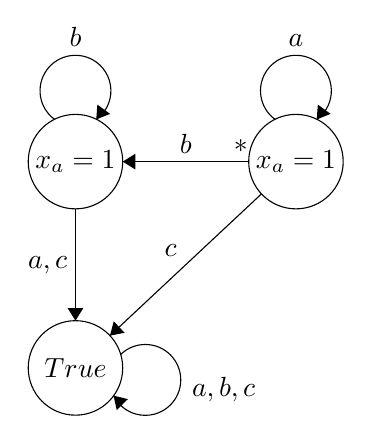
\begin{tikzpicture}[scale=0.2]
    \tikzstyle{every node}+=[inner sep=0pt]
    \draw [black] (17.2,-19.9) circle (3);
    \draw (17.2,-19.9) node {$x_a=1$};
    \draw [black] (17.2,-33) circle (3);
    \draw (17.2,-33) node {$True$};
    \draw [black] (31.2,-19.9) circle (3);
    \draw (31.2,-19.9) node {$x_a=1$};
    \draw (27.7,-18.9) node {$*$};
    \draw [black] (15.877,-17.22) arc (234:-54:2.25);
    \draw (17.2,-12.65) node [above] {$b$};
    \fill [black] (18.52,-17.22) -- (19.4,-16.87) -- (18.59,-16.28);
    \draw [black] (17.2,-22.9) -- (17.2,-30);
    \fill [black] (17.2,-30) -- (17.7,-29.2) -- (16.7,-29.2);
    \draw (16.7,-26.45) node [left] {$a,c$};
    \draw [black] (29.877,-17.22) arc (234:-54:2.25);
    \draw (31.2,-12.65) node [above] {$a$};
    \fill [black] (32.52,-17.22) -- (33.4,-16.87) -- (32.59,-16.28);
    \draw [black] (28.2,-19.9) -- (20.2,-19.9);
    \fill [black] (20.2,-19.9) -- (21,-20.4) -- (21,-19.4);
    \draw (24.2,-19.4) node [above] {$b$};
    \draw [black] (29.01,-21.95) -- (19.39,-30.95);
    \fill [black] (19.39,-30.95) -- (20.32,-30.77) -- (19.63,-30.04);
    \draw (23.24,-25.97) node [above] {$c$};
    \draw [black] (20.065,-32.15) arc (134.26569:-153.73431:2.25);
    \draw (24.57,-34.38) node [right] {$a,b,c$};
    \fill [black] (19.62,-34.76) -- (19.82,-35.68) -- (20.53,-34.98);
    \end{tikzpicture}
    \end{center}

    \pagebreak
    \item Representation of model \textbf{M'}:

    \begin{center}
    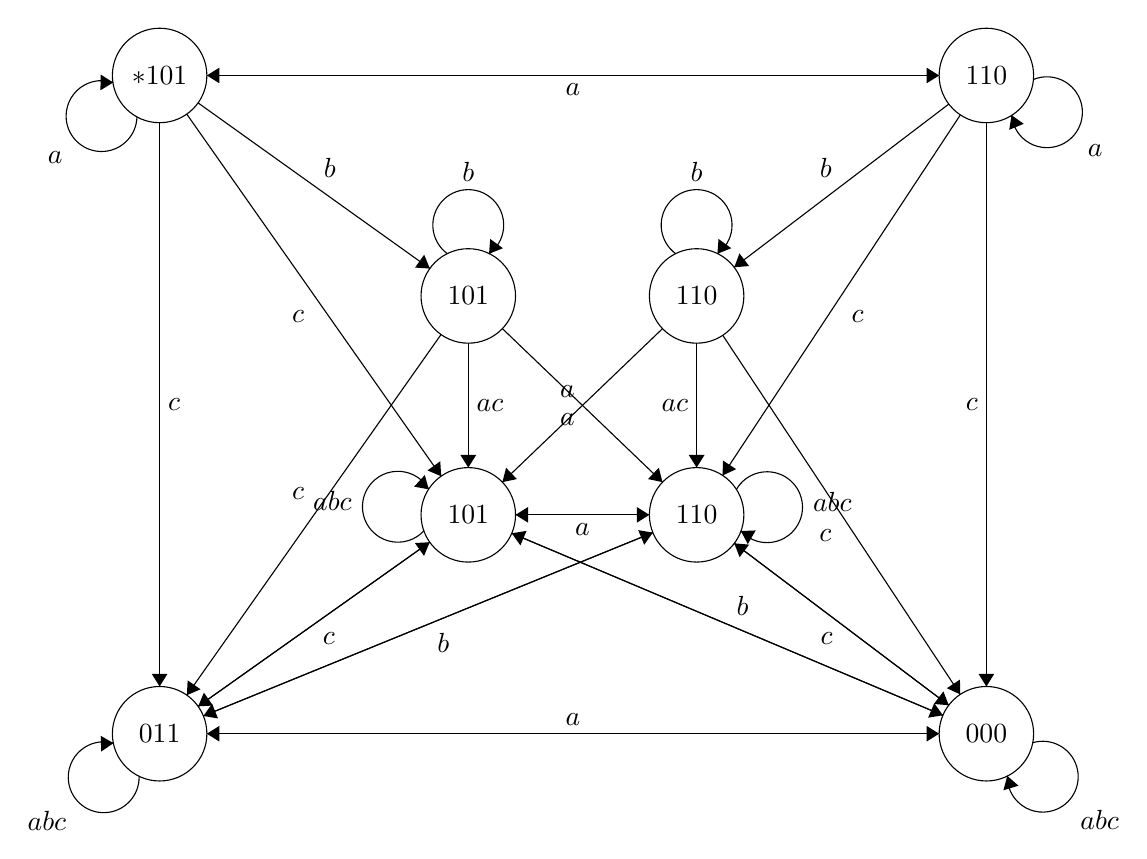
\begin{tikzpicture}[scale=0.2]
    \tikzstyle{every node}+=[inner sep=0pt]
    \draw [black] (65.3,-48.5) circle (3);
    \draw (65.3,-48.5) node {$000$};
    \draw [black] (32.4,-34.6) circle (3);
    \draw (32.4,-34.6) node {$101$};
    \draw [black] (46.9,-34.6) circle (3);
    \draw (46.9,-34.6) node {$110$};
    \draw [black] (12.8,-48.5) circle (3);
    \draw (12.8,-48.5) node {$011$};
    \draw [black] (32.4,-20.7) circle (3);
    \draw (32.4,-20.7) node {$101$};
    \draw [black] (46.9,-20.7) circle (3);
    \draw (46.9,-20.7) node {$110$};
    \draw [black] (65.3,-6.7) circle (3);
    \draw (65.3,-6.7) node {$110$};
    \draw [black] (12.8,-6.7) circle (3);
    \draw (12.8,-6.7) node {$*101$};
    \draw [black] (62.54,-47.33) -- (35.16,-35.77);
    \fill [black] (35.16,-35.77) -- (35.71,-36.54) -- (36.1,-35.62);
    \draw (49.82,-41.04) node [above] {$b$};
    \draw [black] (35.16,-35.77) -- (62.54,-47.33);
    \fill [black] (62.54,-47.33) -- (61.99,-46.56) -- (61.6,-47.48);
    \draw [black] (15.25,-46.76) -- (29.95,-36.34);
    \fill [black] (29.95,-36.34) -- (29.01,-36.39) -- (29.59,-37.21);
    \draw (23.55,-42.05) node [below] {$c$};
    \draw [black] (29.95,-36.34) -- (15.25,-46.76);
    \fill [black] (15.25,-46.76) -- (16.19,-46.71) -- (15.61,-45.89);
    \draw [black] (35.4,-34.6) -- (43.9,-34.6);
    \fill [black] (43.9,-34.6) -- (43.1,-34.1) -- (43.1,-35.1);
    \draw (39.65,-35.1) node [below] {$a$};
    \draw [black] (43.9,-34.6) -- (35.4,-34.6);
    \fill [black] (35.4,-34.6) -- (36.2,-35.1) -- (36.2,-34.1);
    \draw [black] (15.8,-48.5) -- (62.3,-48.5);
    \fill [black] (62.3,-48.5) -- (61.5,-48) -- (61.5,-49);
    \draw (39.05,-48) node [above] {$a$};
    \draw [black] (62.3,-48.5) -- (15.8,-48.5);
    \fill [black] (15.8,-48.5) -- (16.6,-49) -- (16.6,-48);
    \draw [black] (15.58,-47.37) -- (44.12,-35.73);
    \fill [black] (44.12,-35.73) -- (43.19,-35.57) -- (43.57,-36.5);
    \draw (30.81,-42.07) node [below] {$b$};
    \draw [black] (44.12,-35.73) -- (15.58,-47.37);
    \fill [black] (15.58,-47.37) -- (16.51,-47.53) -- (16.13,-46.6);
    \draw [black] (62.91,-46.69) -- (49.29,-36.41);
    \fill [black] (49.29,-36.41) -- (49.63,-37.29) -- (50.23,-36.49);
    \draw (55.15,-42.05) node [below] {$c$};
    \draw [black] (49.29,-36.41) -- (62.91,-46.69);
    \fill [black] (62.91,-46.69) -- (62.57,-45.81) -- (61.97,-46.61);
    \draw [black] (68.233,-49.073) arc (106.67475:-181.32525:2.25);
    \draw (71.24,-54) node [right] {$abc$};
    \fill [black] (66.63,-51.18) -- (66.38,-52.09) -- (67.34,-51.8);
    \draw [black] (11.497,-51.189) arc (1.88392:-286.11608:2.25);
    \draw (6.9,-54.06) node [left] {$abc$};
    \fill [black] (9.87,-49.1) -- (9.06,-48.63) -- (9.09,-49.63);
    \draw [black] (49.421,-32.996) arc (150.19:-137.81:2.25);
    \draw (54.26,-33.77) node [right] {$abc$};
    \fill [black] (49.71,-35.63) -- (50.15,-36.46) -- (50.65,-35.59);
    \draw [black] (29.587,-35.607) arc (317.43022:29.43022:2.25);
    \draw (25.03,-33.71) node [left] {$abc$};
    \fill [black] (29.89,-32.98) -- (29.64,-32.07) -- (28.96,-32.81);
    \draw [black] (34.57,-22.78) -- (44.73,-32.52);
    \fill [black] (44.73,-32.52) -- (44.5,-31.61) -- (43.81,-32.33);
    \draw (38.69,-28.13) node [below] {$a$};
    \draw [black] (45.577,-18.02) arc (234:-54:2.25);
    \draw (46.9,-13.45) node [above] {$b$};
    \fill [black] (48.22,-18.02) -- (49.1,-17.67) -- (48.29,-17.08);
    \draw [black] (44.73,-22.78) -- (34.57,-32.52);
    \fill [black] (34.57,-32.52) -- (35.49,-32.33) -- (34.8,-31.61);
    \draw (38.69,-27.17) node [above] {$a$};
    \draw [black] (31.077,-18.02) arc (234:-54:2.25);
    \draw (32.4,-13.45) node [above] {$b$};
    \fill [black] (33.72,-18.02) -- (34.6,-17.67) -- (33.79,-17.08);
    \draw [black] (32.4,-23.7) -- (32.4,-31.6);
    \fill [black] (32.4,-31.6) -- (32.9,-30.8) -- (31.9,-30.8);
    \draw (32.9,-27.65) node [right] {$ac$};
    \draw [black] (15.24,-8.44) -- (29.96,-18.96);
    \fill [black] (29.96,-18.96) -- (29.6,-18.08) -- (29.02,-18.9);
    \draw (23.6,-13.2) node [above] {$b$};
    \draw [black] (62.91,-8.52) -- (49.29,-18.88);
    \fill [black] (49.29,-18.88) -- (50.23,-18.8) -- (49.62,-18);
    \draw (55.1,-13.2) node [above] {$b$};
    \draw [black] (46.9,-23.7) -- (46.9,-31.6);
    \fill [black] (46.9,-31.6) -- (47.4,-30.8) -- (46.4,-30.8);
    \draw (46.4,-27.65) node [left] {$ac$};
    \draw [black] (68.277,-6.96) arc (112.73627:-175.26373:2.25);
    \draw (71.71,-11.47) node [right] {$a$};
    \fill [black] (66.9,-9.22) -- (66.75,-10.15) -- (67.67,-9.77);
    \draw [black] (11.361,-9.319) arc (-1.04687:-289.04687:2.25);
    \draw (6.67,-11.93) node [left] {$a$};
    \fill [black] (9.85,-7.15) -- (9.06,-6.64) -- (9.04,-7.64);
    \draw [black] (15.8,-6.7) -- (62.3,-6.7);
    \fill [black] (62.3,-6.7) -- (61.5,-6.2) -- (61.5,-7.2);
    \draw (39.05,-7.2) node [below] {$a$};
    \draw [black] (62.3,-6.7) -- (15.8,-6.7);
    \fill [black] (15.8,-6.7) -- (16.6,-7.2) -- (16.6,-6.2);
    \draw [black] (12.8,-9.7) -- (12.8,-45.5);
    \fill [black] (12.8,-45.5) -- (13.3,-44.7) -- (12.3,-44.7);
    \draw (13.3,-27.6) node [right] {$c$};
    \draw [black] (14.52,-9.15) -- (30.68,-32.15);
    \fill [black] (30.68,-32.15) -- (30.62,-31.2) -- (29.81,-31.78);
    \draw (22.01,-22.01) node [left] {$c$};
    \draw [black] (30.67,-23.15) -- (14.53,-46.05);
    \fill [black] (14.53,-46.05) -- (15.4,-45.68) -- (14.58,-45.11);
    \draw (22.01,-33.23) node [left] {$c$};
    \draw [black] (65.3,-9.7) -- (65.3,-45.5);
    \fill [black] (65.3,-45.5) -- (65.8,-44.7) -- (64.8,-44.7);
    \draw (64.8,-27.6) node [left] {$c$};
    \draw [black] (63.65,-9.2) -- (48.55,-32.1);
    \fill [black] (48.55,-32.1) -- (49.41,-31.7) -- (48.57,-31.15);
    \draw (56.71,-21.98) node [right] {$c$};
    \draw [black] (48.56,-23.2) -- (63.64,-46);
    \fill [black] (63.64,-46) -- (63.62,-45.06) -- (62.79,-45.61);
    \draw (55.49,-35.93) node [left] {$c$};
    \end{tikzpicture}
    \end{center}

    \item Representation of event model \textbf{$\Sigma$'}:

    \begin{center}
    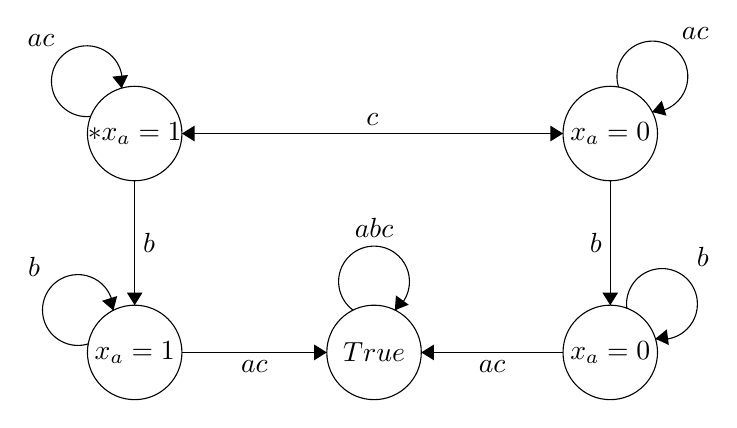
\begin{tikzpicture}[scale=0.2]
    \tikzstyle{every node}+=[inner sep=0pt]
    \draw [black] (18.3,-23.4) circle (3);
    \draw (18.3,-23.4) node {$x_a=1$};
    \draw [black] (48.5,-9.5) circle (3);
    \draw (48.5,-9.5) node {$x_a=0$};
    \draw [black] (33.5,-23.4) circle (3);
    \draw (33.5,-23.4) node {$True$};
    \draw [black] (18.3,-9.5) circle (3);
    \draw (18.3,-9.5) node {$*x_a=1$};
    \draw [black] (48.5,-23.4) circle (3);
    \draw (48.5,-23.4) node {$x_a=0$};
    \draw [black] (15.362,-22.855) arc (287.21852:-0.78148:2.25);
    \draw (12.32,-17.96) node [left] {$b$};
    \fill [black] (16.95,-20.74) -- (17.19,-19.82) -- (16.23,-20.12);
    \draw [black] (49.029,-6.559) arc (197.52793:-90.47207:2.25);
    \draw (53.9,-3.57) node [above] {$ac$};
    \fill [black] (51.16,-8.13) -- (52.07,-8.37) -- (51.77,-7.41);
    \draw [black] (32.177,-20.72) arc (234:-54:2.25);
    \draw (33.5,-16.15) node [above] {$abc$};
    \fill [black] (34.82,-20.72) -- (35.7,-20.37) -- (34.89,-19.78);
    \draw [black] (21.3,-23.4) -- (30.5,-23.4);
    \fill [black] (30.5,-23.4) -- (29.7,-22.9) -- (29.7,-23.9);
    \draw (25.9,-23.9) node [below] {$ac$};
    \draw [black] (18.3,-12.5) -- (18.3,-20.4);
    \fill [black] (18.3,-20.4) -- (18.8,-19.6) -- (17.8,-19.6);
    \draw (18.8,-16.45) node [right] {$b$};
    \draw [black] (15.516,-8.413) arc (276.39744:-11.60256:2.25);
    \draw (12.35,-4.03) node [above] {$ac$};
    \fill [black] (17.47,-6.63) -- (17.88,-5.78) -- (16.88,-5.89);
    \draw [black] (21.3,-9.5) -- (45.5,-9.5);
    \fill [black] (45.5,-9.5) -- (44.7,-9) -- (44.7,-10);
    \draw [black] (45.5,-9.5) -- (21.3,-9.5);
    \fill [black] (21.3,-9.5) -- (22.1,-10) -- (22.1,-9);
    \draw (33.4,-9) node [above] {$c$};
    \draw [black] (48.5,-12.5) -- (48.5,-20.4);
    \fill [black] (48.5,-20.4) -- (49,-19.6) -- (48,-19.6);
    \draw (48,-16.45) node [left] {$b$};
    \draw [black] (49.552,-20.603) arc (187.12:-100.88:2.25);
    \draw (53.96,-17.32) node [right] {$b$};
    \fill [black] (51.36,-22.53) -- (52.22,-22.93) -- (52.09,-21.94);
    \draw [black] (45.5,-23.4) -- (36.5,-23.4);
    \fill [black] (36.5,-23.4) -- (37.3,-23.9) -- (37.3,-22.9);
    \draw (41,-23.9) node [below] {$ac$};
    \end{tikzpicture}
    \end{center}

    \pagebreak

    \item The update product of the two models \textbf{M''} = \textbf{M}
    $\bigotimes$ \textbf{$\Sigma$'} : \\

    \begin{center}
    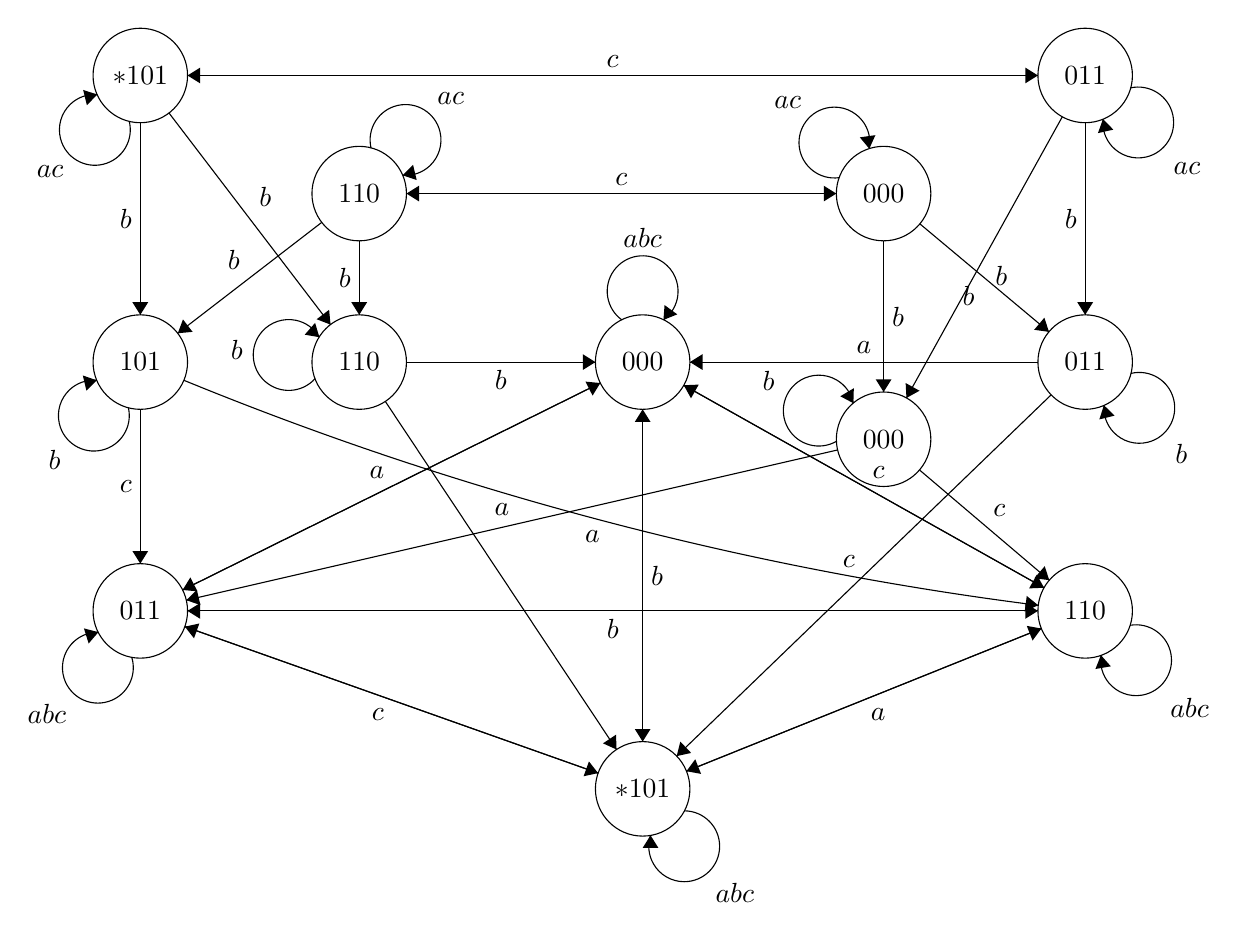
\begin{tikzpicture}[scale=0.2]
    \tikzstyle{every node}+=[inner sep=0pt]
    \draw [black] (7.3,-38.9) circle (3);
    \draw (7.3,-38.9) node {$011$};
    \draw [black] (67.3,-38.9) circle (3);
    \draw (67.3,-38.9) node {$110$};
    \draw [black] (39.2,-50.2) circle (3);
    \draw (39.2,-50.2) node {$*101$};
    \draw [black] (39.2,-23.1) circle (3);
    \draw (39.2,-23.1) node {$000$};
    \draw [black] (21.2,-23.1) circle (3);
    \draw (21.2,-23.1) node {$110$};
    \draw [black] (21.2,-12.4) circle (3);
    \draw (21.2,-12.4) node {$110$};
    \draw [black] (7.3,-4.9) circle (3);
    \draw (7.3,-4.9) node {$*101$};
    \draw [black] (7.3,-23.1) circle (3);
    \draw (7.3,-23.1) node {$101$};
    \draw [black] (54.5,-12.4) circle (3);
    \draw (54.5,-12.4) node {$000$};
    \draw [black] (54.5,-28) circle (3);
    \draw (54.5,-28) node {$000$};
    \draw [black] (67.3,-4.9) circle (3);
    \draw (67.3,-4.9) node {$011$};
    \draw [black] (67.3,-23.1) circle (3);
    \draw (67.3,-23.1) node {$011$};
    \draw [black] (10.3,-38.9) -- (64.3,-38.9);
    \fill [black] (64.3,-38.9) -- (63.5,-38.4) -- (63.5,-39.4);
    \draw (37.3,-39.4) node [below] {$b$};
    \draw [black] (64.3,-38.9) -- (10.3,-38.9);
    \fill [black] (10.3,-38.9) -- (11.1,-39.4) -- (11.1,-38.4);
    \draw [black] (70.145,-39.815) arc (99.89532:-188.10468:2.25);
    \draw (72.67,-45.07) node [right] {$abc$};
    \fill [black] (68.3,-41.71) -- (67.95,-42.59) -- (68.93,-42.42);
    \draw [black] (6.755,-41.838) arc (17.22775:-270.77225:2.25);
    \draw (1.37,-44.8) node [below] {$abc$};
    \fill [black] (4.64,-40.25) -- (3.72,-40.01) -- (4.02,-40.97);
    \draw [black] (41.98,-49.08) -- (64.52,-40.02);
    \fill [black] (64.52,-40.02) -- (63.59,-39.85) -- (63.96,-40.78);
    \draw (54.15,-45.07) node [below] {$a$};
    \draw [black] (37.877,-20.42) arc (234:-54:2.25);
    \draw (39.2,-15.85) node [above] {$abc$};
    \fill [black] (40.52,-20.42) -- (41.4,-20.07) -- (40.59,-19.48);
    \draw [black] (36.51,-24.43) -- (9.99,-37.57);
    \fill [black] (9.99,-37.57) -- (10.93,-37.66) -- (10.48,-36.77);
    \draw (22.32,-30.5) node [above] {$a$};
    \draw [black] (41.842,-51.596) arc (89.89275:-198.10725:2.25);
    \draw (45.05,-56.17) node [below] {$abc$};
    \fill [black] (39.7,-53.15) -- (39.2,-53.95) -- (40.2,-53.95);
    \draw [black] (36.37,-49.2) -- (10.13,-39.9);
    \fill [black] (10.13,-39.9) -- (10.71,-40.64) -- (11.05,-39.7);
    \draw (22.38,-45.08) node [below] {$c$};
    \draw [black] (41.81,-24.57) -- (64.69,-37.43);
    \fill [black] (64.69,-37.43) -- (64.23,-36.6) -- (63.74,-37.47);
    \draw [black] (39.2,-47.2) -- (39.2,-26.1);
    \fill [black] (39.2,-26.1) -- (38.7,-26.9) -- (39.7,-26.9);
    \draw (39.7,-36.65) node [right] {$b$};
    \draw [black] (39.2,-26.1) -- (39.2,-47.2);
    \fill [black] (39.2,-47.2) -- (39.7,-46.4) -- (38.7,-46.4);
    \draw [black] (9.99,-37.57) -- (36.51,-24.43);
    \fill [black] (36.51,-24.43) -- (35.57,-24.34) -- (36.02,-25.23);
    \draw [black] (64.69,-37.43) -- (41.81,-24.57);
    \fill [black] (41.81,-24.57) -- (42.27,-25.4) -- (42.76,-24.53);
    \draw (54.19,-30.5) node [above] {$c$};
    \draw [black] (18.401,-24.147) arc (318.24444:30.24444:2.25);
    \draw (13.84,-22.33) node [left] {$b$};
    \fill [black] (18.67,-21.52) -- (18.4,-20.61) -- (17.74,-21.36);
    \draw [black] (22.86,-25.6) -- (37.54,-47.7);
    \fill [black] (37.54,-47.7) -- (37.51,-46.76) -- (36.68,-47.31);
    \draw [black] (64.52,-40.02) -- (41.98,-49.08);
    \fill [black] (41.98,-49.08) -- (42.91,-49.25) -- (42.54,-48.32);
    \draw [black] (10.13,-39.9) -- (36.37,-49.2);
    \fill [black] (36.37,-49.2) -- (35.79,-48.46) -- (35.45,-49.4);
    \draw [black] (24.2,-23.1) -- (36.2,-23.1);
    \fill [black] (36.2,-23.1) -- (35.4,-22.6) -- (35.4,-23.6);
    \draw (30.2,-23.6) node [below] {$b$};
    \draw [black] (9.12,-7.28) -- (19.38,-20.72);
    \fill [black] (19.38,-20.72) -- (19.29,-19.78) -- (18.5,-20.38);
    \draw (14.82,-12.6) node [right] {$b$};
    \draw [black] (21.2,-15.4) -- (21.2,-20.1);
    \fill [black] (21.2,-20.1) -- (21.7,-19.3) -- (20.7,-19.3);
    \draw (20.7,-17.75) node [left] {$b$};
    \draw [black] (21.952,-9.508) arc (193.15624:-94.84376:2.25);
    \draw (27.01,-6.8) node [above] {$ac$};
    \fill [black] (23.95,-11.24) -- (24.85,-11.54) -- (24.62,-10.57);
    \draw [black] (6.596,-7.804) arc (14.10535:-273.89465:2.25);
    \draw (1.57,-10.57) node [below] {$ac$};
    \fill [black] (4.57,-6.11) -- (3.67,-5.82) -- (3.91,-6.79);
    \draw [black] (6.542,-25.991) arc (13.03983:-274.96017:2.25);
    \draw (1.86,-28.69) node [below] {$b$};
    \fill [black] (4.54,-24.26) -- (3.65,-23.95) -- (3.88,-24.92);
    \draw [black] (18.82,-14.23) -- (9.68,-21.27);
    \fill [black] (9.68,-21.27) -- (10.62,-21.18) -- (10.01,-20.39);
    \draw (13.24,-17.25) node [above] {$b$};
    \draw [black] (7.3,-7.9) -- (7.3,-20.1);
    \fill [black] (7.3,-20.1) -- (7.8,-19.3) -- (6.8,-19.3);
    \draw (6.8,-14) node [left] {$b$};
    \draw [black] (64.321,-38.544) arc (-97.20868:-112.29725:213.657);
    \fill [black] (64.32,-38.54) -- (63.59,-37.95) -- (63.46,-38.94);
    \draw (36.01,-33.75) node [below] {$a$};
    \draw [black] (7.3,-26.1) -- (7.3,-35.9);
    \fill [black] (7.3,-35.9) -- (7.8,-35.1) -- (6.8,-35.1);
    \draw (6.8,-31) node [left] {$c$};
    \draw [black] (51.514,-28.126) arc (300.14714:12.14714:2.25);
    \draw (47.6,-24.28) node [left] {$b$};
    \fill [black] (52.58,-25.71) -- (52.61,-24.76) -- (51.75,-25.27);
    \draw [black] (70.2,-23.821) arc (103.76817:-184.23183:2.25);
    \draw (73,-28.9) node [right] {$b$};
    \fill [black] (68.49,-25.84) -- (68.2,-26.74) -- (69.17,-26.5);
    \draw [black] (51.688,-11.388) arc (277.92756:-10.07244:2.25);
    \draw (48.41,-7.06) node [above] {$ac$};
    \fill [black] (53.59,-9.55) -- (53.98,-8.69) -- (52.99,-8.83);
    \draw [black] (70.182,-5.688) arc (102.44086:-185.55914:2.25);
    \draw (72.89,-10.83) node [right] {$ac$};
    \fill [black] (68.43,-7.67) -- (68.11,-8.56) -- (69.09,-8.34);
    \draw [black] (56.78,-29.95) -- (65.02,-36.95);
    \fill [black] (65.02,-36.95) -- (64.73,-36.06) -- (64.08,-36.82);
    \draw (61.85,-32.96) node [above] {$c$};
    \draw [black] (51.58,-28.68) -- (10.22,-38.22);
    \fill [black] (10.22,-38.22) -- (11.12,-38.53) -- (10.89,-37.56);
    \draw (30.27,-32.88) node [above] {$a$};
    \draw [black] (64.3,-23.1) -- (42.2,-23.1);
    \fill [black] (42.2,-23.1) -- (43,-23.6) -- (43,-22.6);
    \draw (53.25,-22.6) node [above] {$a$};
    \draw [black] (65.14,-25.18) -- (41.36,-48.12);
    \fill [black] (41.36,-48.12) -- (42.28,-47.92) -- (41.59,-47.2);
    \draw (52.29,-36.17) node [above] {$c$};
    \draw [black] (54.5,-15.4) -- (54.5,-25);
    \fill [black] (54.5,-25) -- (55,-24.2) -- (54,-24.2);
    \draw (55,-20.2) node [right] {$b$};
    \draw [black] (67.3,-7.9) -- (67.3,-20.1);
    \fill [black] (67.3,-20.1) -- (67.8,-19.3) -- (66.8,-19.3);
    \draw (66.8,-14) node [left] {$b$};
    \draw [black] (65.85,-7.52) -- (55.95,-25.38);
    \fill [black] (55.95,-25.38) -- (56.78,-24.92) -- (55.9,-24.43);
    \draw (61.57,-17.65) node [right] {$b$};
    \draw [black] (56.8,-14.32) -- (65,-21.18);
    \fill [black] (65,-21.18) -- (64.71,-20.28) -- (64.06,-21.05);
    \draw (59.89,-18.24) node [below] {$b$};
    \draw [black] (24.2,-12.4) -- (51.5,-12.4);
    \fill [black] (51.5,-12.4) -- (50.7,-11.9) -- (50.7,-12.9);
    \draw (37.85,-11.9) node [above] {$c$};
    \draw [black] (51.5,-12.4) -- (24.2,-12.4);
    \fill [black] (24.2,-12.4) -- (25,-12.9) -- (25,-11.9);
    \draw [black] (64.3,-4.9) -- (10.3,-4.9);
    \fill [black] (10.3,-4.9) -- (11.1,-5.4) -- (11.1,-4.4);
    \draw (37.3,-4.4) node [above] {$c$};
    \draw [black] (10.3,-4.9) -- (64.3,-4.9);
    \fill [black] (64.3,-4.9) -- (63.5,-4.4) -- (63.5,-5.4);
    \end{tikzpicture}
    \end{center}



\end{enumerate}

\newpage

%%%%%%%%%%%%%%%%
%% Exercise 3 %%
%%%%%%%%%%%%%%%%
\section*{Exercise 3}
Each of two children, Alice and Bob, has a natural number written in the \textit{back of his/her head}. Let $n_a \in \{0, 1, 2, \dots\}$ be Alice's number and $n_b \in \{0, 1, 2, \dots\}$ be Bob's number. It is common knowledge that: (i) \textit{no child can see his/her own number}, (ii) Alice stands in the back of Bob, so \textit{she can see Bob's number $n_b$, but Bob cannot see any of the numbers}, and (iii) one of the numbers is the immediate successor of the other (in any order): i.e. either $n_a = n_b + 1$ or $n_b = n_a + 1$.
In the following, each of the children will be asked a number of questions, which they are required to answer publicly and truthfully.

\begin{enumerate}
    \item \textit{How many possible worlds} are there (that are consistent with the story above)?
    
   	There are infinite possible worlds.

    \item \textit{Represent} \textbf{(draw) the above situation as an \textit{epistemic model} M$_1$}, with two agents ($a$ for Alice, $b$ for Bob), using pairs of numbers ($n_a$,$n_b$) as ``names'' for the possible worlds. \textbf{Draw the epistemic accessibility  relations} for each agent, but do \textit{not} worry about the valuation (yet), since no atomic sentences are given yet.

	For simplicity we skipped the loops (every world has an $a$- and $b$-arrow to itself) and we skipped a lot of $b$-arrows (every world has a $b$-arrow to every other world).
    \begin{center}
    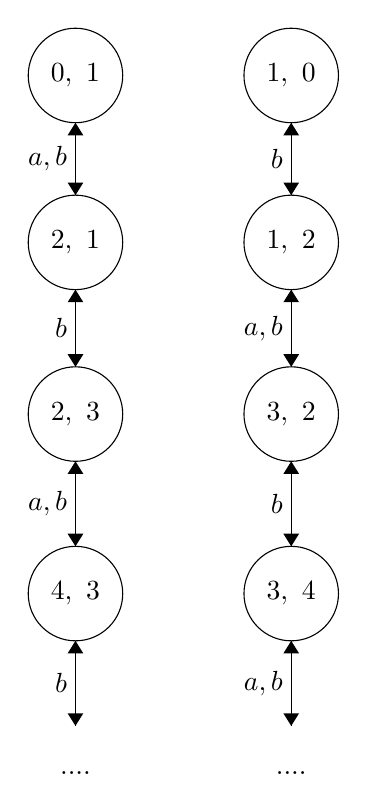
\begin{tikzpicture}[scale=0.2]
	    \tikzstyle{every node}+=[inner sep=0pt]
	    \draw [black] (25,-11.7) circle (3);
	    \draw (25,-11.7) node {$0,\mbox{ }1$};
	    \draw [black] (38.7,-11.7) circle (3);
	    \draw (38.7,-11.7) node {$1,\mbox{ }0$};
	    \draw [black] (38.7,-22.3) circle (3);
	    \draw (38.7,-22.3) node {$1,\mbox{ }2$};
	    \draw [black] (25,-22.3) circle (3);
	    \draw (25,-22.3) node {$2,\mbox{ }1$};
	    \draw [black] (25,-33.2) circle (3);
	    \draw (25,-33.2) node {$2,\mbox{ }3$};
	    \draw [black] (38.7,-33.2) circle (3);
	    \draw (38.7,-33.2) node {$3,\mbox{ }2$};
	    \draw [black] (25,-44.6) circle (3);
	    \draw (25,-44.6) node {$4,\mbox{ }3$};
	    \draw [black] (38.7,-44.6) circle (3);
	    \draw (38.7,-44.6) node {$3,\mbox{ }4$};
	    \draw (25,-56) node {$....$};
	    \draw (38.7,-56) node {$....$};
	    \draw [black] (25,-14.7) -- (25,-19.3);
	    \fill [black] (25,-19.3) -- (25.5,-18.5) -- (24.5,-18.5);
	    \draw (24.5,-17) node [left] {$a, b$};
	    \draw [black] (38.7,-14.7) -- (38.7,-19.3);
	    \fill [black] (38.7,-19.3) -- (39.2,-18.5) -- (38.2,-18.5);
	    \draw (38.2,-17) node [left] {$b$};
	    \draw [black] (38.7,-25.3) -- (38.7,-30.2);
	    \fill [black] (38.7,-30.2) -- (39.2,-29.4) -- (38.2,-29.4);
	    \draw (38.2,-27.75) node [left] {$a, b$};
	    \draw [black] (25,-25.3) -- (25,-30.2);
	    \fill [black] (25,-30.2) -- (25.5,-29.4) -- (24.5,-29.4);
	    \draw (24.5,-27.75) node [left] {$b$};
	    \draw [black] (38.7,-36.2) -- (38.7,-41.6);
	    \fill [black] (38.7,-41.6) -- (39.2,-40.8) -- (38.2,-40.8);
	    \draw (38.2,-38.9) node [left] {$b$};
	    \draw [black] (38.7,-47.6) -- (38.7,-53);
	    \fill [black] (38.7,-53) -- (39.2,-52.2) -- (38.2,-52.2);
	    \draw (38.2,-50.3) node [left] {$a, b$};
	    \draw [black] (25,-47.6) -- (25,-53);
	    \fill [black] (25,-53) -- (25.5,-52.2) -- (24.5,-52.2);
	    \draw (24.5,-50.3) node [left] {$b$};
	    \draw [black] (25,-36.2) -- (25,-41.6);
	    \fill [black] (25,-41.6) -- (25.5,-40.8) -- (24.5,-40.8);
	    \draw (24.5,-38.9) node [left] {$a, b$};
	    \draw [black] (25,-19.3) -- (25,-14.7);
	    \fill [black] (25,-14.7) -- (24.5,-15.5) -- (25.5,-15.5);
	    \draw [black] (38.7,-19.3) -- (38.7,-14.7);
	    \fill [black] (38.7,-14.7) -- (38.2,-15.5) -- (39.2,-15.5);
	    \draw [black] (38.7,-30.2) -- (38.7,-25.3);
	    \fill [black] (38.7,-25.3) -- (38.2,-26.1) -- (39.2,-26.1);
	    \draw [black] (25,-30.2) -- (25,-25.3);
	    \fill [black] (25,-25.3) -- (24.5,-26.1) -- (25.5,-26.1);
	    \draw [black] (25,-41.6) -- (25,-36.2);
	    \fill [black] (25,-36.2) -- (24.5,-37) -- (25.5,-37);
	    \draw [black] (38.7,-41.6) -- (38.7,-36.2);
	    \fill [black] (38.7,-36.2) -- (38.2,-37) -- (39.2,-37);
	    \draw [black] (38.7,-53) -- (38.7,-47.6);
	    \fill [black] (38.7,-47.6) -- (38.2,-48.4) -- (39.2,-48.4);
	    \draw [black] (25,-53) -- (25,-47.6);
	    \fill [black] (25,-47.6) -- (24.5,-48.4) -- (25.5,-48.4);
    \end{tikzpicture}
    \end{center}

    \item For your model, consider now the following \textit{four atomic sentences} $0_a, 0_b, 1_a, 1_b$. Here, $0_a$ means ``Alice's number is equal to 0'' (i.e. $n_a = 0$), and $0_b$ means ``Bob's number is equal to 0'' (i.e. $n_b = 0$); $1_a$ means ``Alice's number is equal to 1'' (i.e. $n_a = 1$), and $1_b$ means ``Bob's number is equal to 1'' (i.e. $n_b = 1$). \textbf{Specify the valuation for these atomic sentences} in the above model.
    
    We only learned how to valuate worlds, and the valuation of a world is the set of basic facts that are true in that world. So when we only consider the four atomic sentences above, we have as valuations:
    
    \begin{itemize}[label={}]
    	\item $\nu((0, 1))= \{0_a, 1_b\}$
    	\item $\nu((1, 0))= \{1_a, 0_b\}$
    	\item $\nu((2, 1))= \{1_b\}$
    	\item $\nu((1, 2))= \{1_a\}$
    	\item in all other worlds $v$: $\nu(v) = \emptyset$
    \end{itemize}
    
    If we assume ``valuation of an atomic sentence'' means ``specify the set of worlds in which the atomic sentence is true'', then the valuations are:
    
    \begin{itemize}[label={}]
    	\item $\nu(0_a)= \{(0, 1)\}$
    	\item $\nu(0_b)= \{(1, 0)\}$
    	\item $\nu(1_a)= \{(1, 0), (1, 2)\}$
    	\item $\nu(1_b)= \{(0, 1), (2, 1)\}$
    \end{itemize}    
    
    \item Alice is asked the following question: \textit{``Do you know whether your own number is equal to $0$ or not, and if so then which of the two?''} So her answers can be: (a) \textit{I don't know}, (b) \textit{I know that my number is equal to $0$}, or (c) \textit{I know that my number is NOT equal to $0$}.
    
    Let us suppose that in fact \textit{Alice answers (c) ``I know that my number is NOT equal to $0$''}.
    
    \textbf{Write down a sentence $\varphi$ in epistemic logic that expresses her \textit{answer}}.
    
    $\varphi$ = K$_a(\neg 0_a)$
    
    \item Interpreting the above answer as a truthful public announcement $!\varphi$ of the sentence written in the previous part, \textbf{represent (draw) the updated model M$_2$ = M$_1^{!\varphi}$ after this public announcement}.
    
    For simplicity we skipped the loops (every world has an $a$- and $b$-arrow to itself) and we skipped a lot of $b$-arrows (every world has a $b$-arrow to every other world).
    \begin{center}
    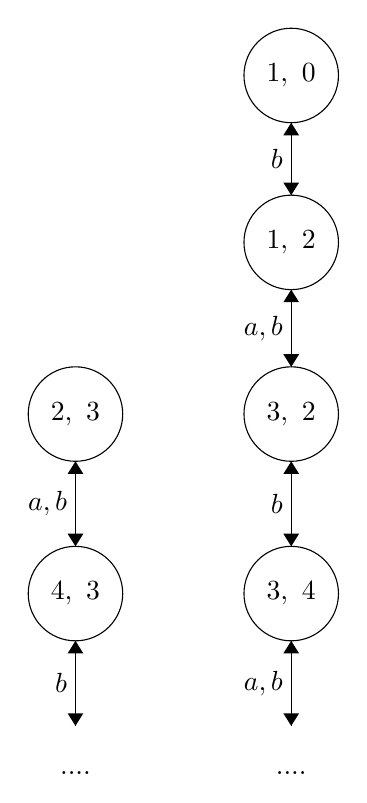
\begin{tikzpicture}[scale=0.2]
	    \tikzstyle{every node}+=[inner sep=0pt]
	    \draw [black] (38.7,-11.7) circle (3);
	    \draw (38.7,-11.7) node {$1,\mbox{ }0$};
	    \draw [black] (38.7,-22.3) circle (3);
	    \draw (38.7,-22.3) node {$1,\mbox{ }2$};
	    \draw [black] (25,-33.2) circle (3);
	    \draw (25,-33.2) node {$2,\mbox{ }3$};
	    \draw [black] (38.7,-33.2) circle (3);
	    \draw (38.7,-33.2) node {$3,\mbox{ }2$};
	    \draw [black] (25,-44.6) circle (3);
	    \draw (25,-44.6) node {$4,\mbox{ }3$};
	    \draw [black] (38.7,-44.6) circle (3);
	    \draw (38.7,-44.6) node {$3,\mbox{ }4$};
	    \draw (25,-56) node {$....$};
	    \draw (38.7,-56) node {$....$};
	    \fill [black] (38.7,-19.3) -- (39.2,-18.5) -- (38.2,-18.5);
	    \draw (38.2,-17) node [left] {$b$};
	    \draw [black] (38.7,-25.3) -- (38.7,-30.2);
	    \fill [black] (38.7,-30.2) -- (39.2,-29.4) -- (38.2,-29.4);
	    \draw (38.2,-27.75) node [left] {$a, b$};
	    %\draw [black] (25,-25.3) -- (25,-30.2);
	    %\fill [black] (25,-30.2) -- (25.5,-29.4) -- (24.5,-29.4);
	    %\draw (24.5,-27.75) node [left] {$b$};
	    \draw [black] (38.7,-36.2) -- (38.7,-41.6);
	    \fill [black] (38.7,-41.6) -- (39.2,-40.8) -- (38.2,-40.8);
	    \draw (38.2,-38.9) node [left] {$b$};
	    \draw [black] (38.7,-47.6) -- (38.7,-53);
	    \fill [black] (38.7,-53) -- (39.2,-52.2) -- (38.2,-52.2);
	    \draw (38.2,-50.3) node [left] {$a, b$};
	    \draw [black] (25,-47.6) -- (25,-53);
	    \fill [black] (25,-53) -- (25.5,-52.2) -- (24.5,-52.2);
	    \draw (24.5,-50.3) node [left] {$b$};
	    \draw [black] (25,-36.2) -- (25,-41.6);
	    \fill [black] (25,-41.6) -- (25.5,-40.8) -- (24.5,-40.8);
	    \draw (24.5,-38.9) node [left] {$a, b$};
	    %\draw [black] (25,-19.3) -- (25,-14.7);
	    %\fill [black] (25,-14.7) -- (24.5,-15.5) -- (25.5,-15.5);
	    \draw [black] (38.7,-19.3) -- (38.7,-14.7);
	    \fill [black] (38.7,-14.7) -- (38.2,-15.5) -- (39.2,-15.5);
	    \draw [black] (38.7,-30.2) -- (38.7,-25.3);
	    \fill [black] (38.7,-25.3) -- (38.2,-26.1) -- (39.2,-26.1);
	    %\draw [black] (25,-30.2) -- (25,-25.3);
	    %\fill [black] (25,-25.3) -- (24.5,-26.1) -- (25.5,-26.1);
	    \draw [black] (25,-41.6) -- (25,-36.2);
	    \fill [black] (25,-36.2) -- (24.5,-37) -- (25.5,-37);
	    \draw [black] (38.7,-41.6) -- (38.7,-36.2);
	    \fill [black] (38.7,-36.2) -- (38.2,-37) -- (39.2,-37);
	    \draw [black] (38.7,-53) -- (38.7,-47.6);
	    \fill [black] (38.7,-47.6) -- (38.2,-48.4) -- (39.2,-48.4);
	    \draw [black] (25,-53) -- (25,-47.6);
	    \fill [black] (25,-47.6) -- (24.5,-48.4) -- (25.5,-48.4);
    \end{tikzpicture}
    \end{center}
    
    \item Suppose now that, \textit{after} Alice answered as above, Bob is asked the ``same'' question: \textit{``Do you (Bob) know whether your own number is equal to $0$ or not, and if so then which of the two}?''
    
    \textbf{What will Bob answer}? Also, \textbf{what will be updated model M$_3$ representing the situation after he answers}? Justify your answers!
    
    Bob will answer (a) \textit{I don't know}, because in all worlds of M$_2$ Bob thinks every other world is possible (there are $b$-arrows going from each world to each other world). M$_3$ = M$_2$ (we cannot remove worlds), because there is no world in which Bob's answer (``I don't know'') is false.
    
    \item After the previous round of questions, Alice is now asked the following question: \textit{``Do you know whether your own number is equal to $1$ or not, and if so then which of the two}?'' The asnwers can be: (a) \textit{I don't know}, (b) \textit{I know that my number is equal to $1$}, or (c) \textit{I know that my number is NOT equal to $1$}.
    
	Let us suppose that in fact \textit{Alice answers (a) ``I don't know''}.
	
    \textbf{Write down a sentence $\psi$ in epistemic logic that expresses her \textit{answer}}.
    
    $\psi$ = $\neg$K$_a(1_a) \land \neg$K$_a(\neg 1_a)$
    
    \item Interpreting the above answer as a truthful public announcement $!\psi$ of the sentence written in the previous part, \textbf{represent (draw) the updated model M$_4$ = M$_3^{!\psi}$ after this public announcement}.
    
    \begin{center}
	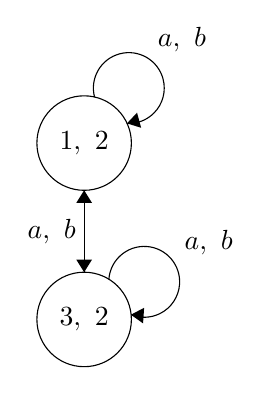
\begin{tikzpicture}[scale=0.2]
		\tikzstyle{every node}+=[inner sep=0pt]
		\draw [black] (37,-17.1) circle (3);
		\draw (37,-17.1) node {$1,\mbox{ }2$};
		\draw [black] (37,-28.3) circle (3);
		\draw (37,-28.3) node {$3,\mbox{ }2$};
		\draw [black] (37,-25.3) -- (37,-20.1);
		\fill [black] (37,-20.1) -- (36.5,-20.9) -- (37.5,-20.9);
		\draw [black] (37,-20.1) -- (37,-25.3);
		\fill [black] (37,-25.3) -- (37.5,-24.5) -- (36.5,-24.5);
		\draw (36.5,-22.7) node [left] {$a,\mbox{ }b$};
		\draw [black] (37.663,-14.186) arc (194.90614:-93.09386:2.25);
		\draw (43.21,-11.37) node [above] {$a,\mbox{ }b$};
		\fill [black] (39.72,-15.85) -- (40.62,-16.13) -- (40.36,-15.17);
		\draw [black] (38.57,-25.757) arc (176.04546:-111.95454:2.25);
		\draw (43.35,-23.42) node [right] {$a,\mbox{ }b$};
		\fill [black] (39.97,-28) -- (40.74,-28.55) -- (40.81,-27.56);
	\end{tikzpicture}
	\end{center}
    
    \item Suppose now that, \textit{after} Alice answered as above, Bob is asked the ``same'' question: \textit{``Do you (Bob) know whether your own number is equal to $1$ or not, and if so then which of the two}?''
    
    \textbf{What will Bob answer}? Also, \textbf{what is his number}? Justify your answers!
    
    Bob will answer (c) \textit{I know that my number is NOT equal to $1$}, because in M$_4$ there is no world in which Bob knows his number is 1 (there is no $b$-arrow to a world where $n_b=1$). $n_b = 2$, because in all possible worlds in M$_4$ Bob's number is 2.

\end{enumerate}


\end{document}


